% vim:ts=2 sw=2 et spell tw=80:

\section{Applications}

As suggested in the previous section, the fact that it is possible to write a
Fourier style expansion of any function on the surface of the sphere is very
useful in many fields of physics and engineering. Here we will present a few of
the most interesting applications we came across during our research.

\subsection{Electroencephalography}

\begin{figure}
  \centering
  \subfigure[EEG Electrodes \label{kugel:fig:eeg-electrodes}]%
    % {\kugelplaceholderfig{.4\linewidth}{5cm}}
    {\includegraphics[width=.45\linewidth, frame]{papers/kugel/figures/electrodes}}
  \qquad
  \subfigure[Gauss' Law \label{kugel:fig:eeg-flux}]%
    {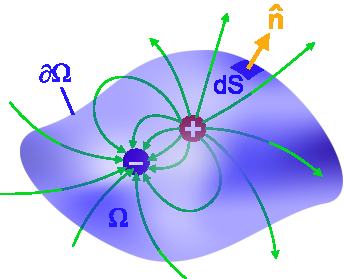
\includegraphics[width=.4\linewidth]{papers/kugel/figures/flux}}
  \caption{
    \label{kugel:fig:eeg}
  }
\end{figure}

To start, we will look at an application that is from the field of medicine:
electroencephalography. The \emph{electroencephalogram} (EEG) is a measurement
of the electrical field on the scalp, which shows the brain's activity, and is
used in many fields of research such as neurology and cognitive psychology.  The
measurement is done by wearing a cap that contains a number of evenly
distributed electrodes, each of which measures the electric potential (voltage)
at their location (figure \ref{kugel:fig:eeg-electrodes}).  To see how this will
relate to the spherical harmonics, we will first quickly recap a bit of physics,
electrodynamics to be precise.


\subsubsection{Electrodynamics}

In section \ref{kugel:sec:construction:eigenvalue} we have shown that the
spherical harmonics arise from the surface spherical Laplacian operator, whose
origin we did not consider too much, which is how mathematicians do their work.
On the contrary, physicists usually do the opposite and start by discussing what
is happening in the real world, since variables represent physical quantities.
So, we will quickly remind that the Laplacian operator does the following to an
electric potential $\phi(x, y, z)$:
\begin{equation*}
  \nabla^2 \phi
  = \nabla \cdot \nabla \phi
  = \nabla \cdot \mathbf{E}
  = \rho / \varepsilon,
  \quad \text{or} \quad
  \iiint_\Omega \nabla \cdot \mathbf{E} \, dv
  = \iint_{\partial \Omega} \mathbf{E} \cdot d\mathbf{s}
  = \Phi / \varepsilon.
\end{equation*}
Put into words: on the left we have the differential form, where we recall that
the Laplacian (which is a second derivative) is the divergence of the gradient.
Unpacking the notation we first see that we have the gradient of the potential,
which is just the electric field $\mathbf{E}$, and then the divergence of said
electric field is proportional to the charge density $\rho$. So, the Laplacian
of the electric potential is the charge density! For those that are more
familiar with the integral form of Maxwell's equation, we have also included an
additional step using the divergence theorem, which brings us to the electric
Flux, which by Gauss' law (shown in the iconic\footnote{Every electrical
engineer has seen this picture so many times that is probably burnt in their
eyes.} figure \ref{kugel:fig:eeg-flux}) equals the net electric charge.

Now, an important observation is that if we switch to spherical coordinates, the
physics does not change. So, the spherical Laplacian $\sphlaplacian$ of the
electric potential $\phi(r, \vartheta, \varphi)$ is still the charge density (in
spherical coordinates). And what about the surface spherical Laplacian
$\surflaplacian$? To that case the physics is also indifferent, the only change
is that the units result is a \emph{surface} charge density $\rho_s$. Thus, we
are done with physics and finally arrive at the engineers' perspective: how can
we use this fact to build something that reads the current flows on the surface
of the brain?

\subsubsection{EEG as Interpolation Problem}

The details of how EEG actually works gets very complicated very quickly, but we
will try our best to give an broad overview of the mathematical machinery that
makes it possible to measure brain waves. The problem neither the physicist nor
the mathematician considered is that we cannot measure the electric field in its
entirety. As show in figure \ref{kugel:fig:eeg-electrodes} the electrodes give
measurements that are only available at discrete locations, and we are thus
missing quite a lot of data. Or in other words, we have an interpolation
problem, which (at this point not so surprisingly) we will show can be solved
using the spherical harmonics.

To solve this new interpolation problem, we will start with a blatantly
engineering assumption: the human head is a sphere of radius $R$, with the value
of $R$ begin the average radius of a human head (which is around 11 cm). So, we
will assume that the potential distribution on the head can be written as a
finite linear combination of spherical harmonics:
\begin{equation*}
  V(\vartheta, \varphi)
    = \sum_{n=1}^N \sum_{m=-n}^n a_{m,n} Y^m_n(\vartheta, \varphi),
\end{equation*}
where the values $a_{m,n}$ are the unknowns of our interpolation problem. Now to
the measurements: we let $\phi_1, \phi_2, \ldots, p_M$ be the measured voltages
at points in space $p_1, p_2, \ldots, p_M$ (position of the electrodes). To
simplify, we will assume that the electrodes are reasonably evenly distributed,
which means that we have no points that are on top of each other or at wildly
different radii from the origin. With that out of the way, we can now write a
minimization problem:
\begin{subequations}
  \begin{align}
    a_{m,n}^* &= \arg \min_{a_{m,n}}
      \int_{\partial S} | \surflaplacian V |^2 \, ds 
      = \int_0^{2\pi} \int_{0}^\pi | \surflaplacian V |^2
        \sin \vartheta \, d\vartheta d\varphi, 
        \label{kugel:eqn:eeg-min} \\
    &\text{under the constraints} \quad V(p_j) = \phi_j
      \quad \text{ for } \quad 1 < j < M.
      \label{kugel:eqn:eeg-min-constraints}
  \end{align}
\end{subequations}
Essentially, with \eqref{kugel:eqn:eeg-min} we are are asking for the solution
to be smooth by minimizing the square of the total curvature (recall that the
surface spherical Laplacian $\surflaplacian$ is a measure of curvature), while
at the same time with \eqref{kugel:eqn:eeg-min-constraints}, we force the
solution to go through the measured points. The latter is the reason why we
needed to assumed that the measurements are at reasonable locations, something
that (as every engineer show know) is not necessarily the case in the real
world! Thus, to solve this problem, we will use the suspiciously convenient fact
that (hint: eigenvalues)
\begin{equation*}
  \surflaplacian V(\vartheta, \varphi)
    = \sum_{n=1}^N \sum_{m=-n}^n a_{m,n}
      \surflaplacian Y^m_n(\vartheta, \varphi)
    = \sum_{n=1}^N \sum_{m=-n}^n a_{m,n}
      n(n+1) Y^m_n(\vartheta, \varphi).
\end{equation*}
So that when substituted into \eqref{kugel:eqn:eeg-min} results in
\begin{align*}
  \int_{\partial S} \left|
    \sum_{n=1}^N \sum_{m=-n}^n n(n+1) a_{m,n}
    Y^m_n(\vartheta, \varphi)
  \right|^2 ds
  = \sum_{m, m'} \sum_{n, n'} a_{m',n'} \overline{a_{m,n}}
    n'(n'+1) n(n+1)
    \underbrace{\int_{\partial S} Y^{m'}_{n'} \overline{Y^m_n} \, ds}_{
      \langle Y^{m'}_{n'}, Y^m_n \rangle
    },
\end{align*}
where we used a ``sloppy'' double sum notation to indicate that we have a bunch
of terms of that form. We did not bother to properly expand the product of
double sums, because we can see that at the end we end up with an inner product
$\langle Y^{m'}_{n'}, Y^m_n \rangle$, which as we know equals $\delta_{m'm}
\delta_{n'n}$, so all of the terms where $n' \neq n$ or $m' \neq m$ can be
dropped and \eqref{kugel:eqn:eeg-min} simplifies down to
\nocite{pascual-marqui_current_1988}
\begin{equation}
  a^*_{m,n} = \arg \min_{a_{m,n}} 
    \sum_{n=1}^N \sum_{m=-n}^n n^2 (n+1)^2 |a_{m,n}|^2.
\end{equation}

At this point, we could continue solving for an analytical solution to the
minimization problem, for example by differentiating with respect to some
$a_{j,k}$, setting that to zero and so forth, but the job of the spherical
harmonics ends here. So, we will not pursue this further, and instead briefly
discuss a few interesting implications and problems. 

\subsubsection{Sampling, Smoothness and Problems}
\nocite{wingeier_spherical_2001, ruffini_spherical_2002}

The most interesting perhaps unforeseen fact is that with this method we are
getting a free (!) spectral analysis, since the coefficients $a_{m,n}$ are the
spectrum of the interpolated electric field $V(\vartheta, \varphi)$. However,
like in the non spherical Fourier transformation, we only get a \emph{finite}
resolution since our measurement are spatially discrete. In fact, if we know the
mean angular inter-electrode distance $\gamma$ we can actually formulate a
Nyquist frequency just like in the usual Fourier theory:
\begin{equation}
  f_N = \frac{\pi}{2T}
  \iff
  n_N = \left\lfloor \frac{\pi}{2\gamma} \right\rfloor.
\end{equation}

Before concluding this overview of EEG, we should point out that in practice
there are about a million problems with this oversimplified approach. We do not
intend to give an in depth explanation (since the authors themselves are not
experts in any of these fields), but there are a few problems that are too big
to ignore, so we will very briefly discuss them now. The first important
real-world problem is that the electrodes are not necessarily at a reasonable
location, so the constraint \eqref{kugel:eqn:eeg-min-constraints} is a bit too
strong, and may end up fitting some noise or disturbances in the measurement. A
simple solution may for example be to introduce a smoothness factor $\lambda >
0$ as follows:
\begin{equation}
  V(\vartheta, \varphi) = \sum_{n=1}^N \sum_{m=-n}^n 
    \frac{a_{m,n}}{1 + \lambda n^2(n+1)^2} Y^m_n(\vartheta, \varphi).
\end{equation}
To find proper smoothness factor $\lambda$, is another problem of its own, thus
we will not discuss it here, since this is getting too long already. Another
important issue is that in the real world, we cannot ``evenly distribute'' the
electrodes on our head. As shown in the image, most of the electrodes are on a
cap, and then there are just a few on the face, and almost none near the jawline
and chin. This not something that can be ignored, and in fact, makes the
analysis much more difficult. Finally, the most obvious problem is that human
heads are not perfect spheres. Here too, it is possible to account for this fact
and model the head with a more complex shape at the cost of making the math
quite unwieldy.

\subsection{Measuring Gravitational Fields}

\subsection{Quantisation of Angular Momentum}
